%%%%%%%%%%%%%%%%%%%%%%%%%%%%%%%%%%%%%%%%%%%%%%%%%%%%%%%%%%%%%%%%%%%%%%%%%%%%%%%%%%%%%%%%%%%%%%%%%%%%%%
%
%   Filename    : chapter_2.tex 
%
%   Description : This file will contain your Review of Related Literature.
%                 
%%%%%%%%%%%%%%%%%%%%%%%%%%%%%%%%%%%%%%%%%%%%%%%%%%%%%%%%%%%%%%%%%%%%%%%%%%%%%%%%%%%%%%%%%%%%%%%%%%%%%%

\chapter{Review of Related Literature}
\label{sec:relatedlit}

This chapter discusses studies of speech training software that have been distributed and used by those with hearing-impairment in order to learn how to speak.

\section{Review of Related Paper}

\subsection{Speech Training Systems}

Speech is not innate for children who are deaf or with a profound hearing loss at birth. The effect of such disability obstructs a child from imitating other people's sounds and comparing the sound he/she may be able to produce with theirs. However, the development which can't be learned through spontaneous speech could be acquired through vision, tactile sensation, and residual hearing. Although, this learning method solely relies on the visual representation of phonemes and through tongue control movements in sustaining the speech movements. Computer-based speech therapy aided programs makes use of visual feedback to allow individuals with profound hearing impairments to evaluate themselves with their produced input compared with an acceptable input. By garnering the attention of the children through drawings and illustrations to demonstrate loudness, pitch contour, spectral distribution, etc., they are able to validate their produced sound \cite{oster:2006:cbs}.

Speech training systems were developed in order to represent feedback to people with profound hearing impairment in a visually appealing manner \cite{oster:2006:cbs}. Other implementations of software address this solution by introducing gamifying elements to allow the software to be used by the direct users or under the assistance of teachers. Methods such as spectrographs, dating since 1947, have also been used to teach speech to children \cite{javkin:1993:msa}. On the other hand, tactile aid focuses on somatosensation; by using vibrators at various parts of the body to indicate numerous elements of speech such as voicing or nasalization \cite{wankhede:2014:dvs}.

Strategies are often required in implementing such systems, especially to Deaf children, who necessitates more efficient methods of instructions compared to children who have the ability to hear. Speech training is efficient if it would be able to allow children to imitate invisible speech articulations, which could not be perceived properly by visual aids \cite{oster:1996:cac}. Oster \citeyear{oster:1996:cac} suggests that for a speech training system to be considered efficient and be able to amplify any possibility for a child to learn, a number of requirements must be achieved:

\begin{itemize}
\item Clear instructions and pedagogical manuals must be created and made available for use with different groups of children.
\item The visual feedback of the child's voice and articulation should be shown immediately and without delay.
\item The aid must be acceptable to the therapist as well as to the child, which means that the aid must be attractive, interesting, easily comprehensible, easy to handle, and motivating.
\item The visual pattern must be natural, logical and easily understandable. This means that training parameters as, e.g., pitch could be shown vertically as pitch variations occur; intensity through the size of an object that becomes larger as a sound becomes louder and smaller as a sound becomes softer; intonation and stress through a continuous red curve; duration could be shown horizontally and voicing through a relationship between voicing and the change of a colour.
\item The aid should provide a contrastive training, that is, the correct model of the therapist and the deviant production of the child are shown simultaneously and compared with each other.
\item The aid should provide a flexible, individual, and structural speech and voice training and give an objective evaluation of the child's training results.
\end{itemize}

A speech training software that provides visual aid will help a hearing-impaired person evaluate and correct his utterance or pronunciation \cite{wankhede:2014:dvs}. Wankhede mentions that how the feedback is presented also affects how hearing-impaired children may improve their pronunciations. The visual feedback must also be shown immediately on the computer screen without delay to prevent confusion to the child. Some children may find some speech training aids as difficult to understand, unnatural, delayed, unattractive, and demotivating. For evaluation of the speech training aid, it should have the acceptance of a speech therapist and as well as of a child, meaning that the system should be appealing, presentable, easy to use, and motivating \cite{wankhede:2014:dvs}.

Aside from visual feedback that are used as aid in speech training software, there is also another type of feedback being used as aid for the hearing-impaired people in speech training - vibrotactile feedback. The Haptic Chair is a project developed by Suranga Nanayakkara, Lonce Wyse, and Elizabeth A. Taylor \citeyear{nanaya:2012:hap}, to help deaf people in speech training by the use of sending vibrotactile feedback to several parts of the body such as palm and fingers.

\pagebreak
\section{Review of Related Software and Types of Feedback}

\subsection{SpeechViewer}

\begin{figure}[h]
    \centering
    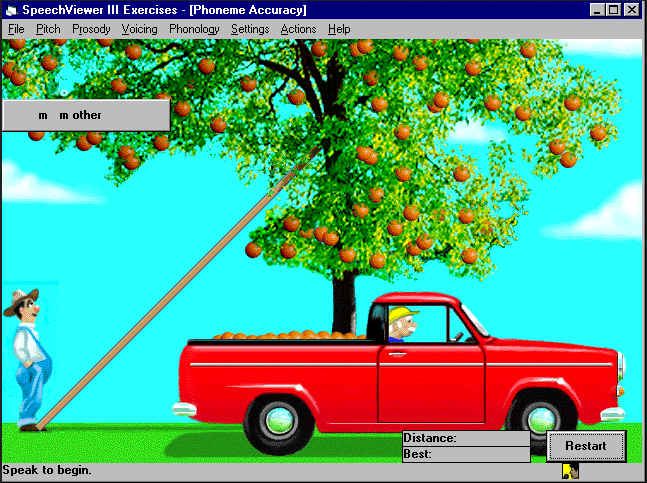
\includegraphics[totalheight=0.2\textheight]{speechviewer.PNG}
    \caption{SpeechViewer III [Online image].}
    \cite{speechviewer3:img}
    \label{fig:speechviewer}
\end{figure}

SpeechViewer III is a software developed by IBM to help the hearing-impaired enhance their vocal skills. It transforms spoken words and sounds into imaginative graphics \cite{speechville:2014:slp}. "SpeechViewer III uses visual and auditory feedback to analyse and improve the speech skills of people who have speech, language or hearing disorders" \cite{kennedy:1998:spv}. The student must be facilitated by a professional in guiding him or her in speech training. The software provides a dozen exercises for the user and also provides immediate and clear feedback. It also gives interest for children as the software gives animated rewards during successful responses.

\subsection{Speech Therapy 5}
"Speech Therapy uses over 70 voice-activated video games to provide real-time reinforcement of a client's attempts to produce changes in pitch, loudness, voiced and unvoiced phonation, voicing onset, maximum phonation time, sound and vowel tracking"\cite{drspeech:1998:st5}. The software is aimed for the development of children, wherein they play interactive games. Immediate animated feedback is displayed to show how well a child performs.

\begin{figure}[h]
    \centering
    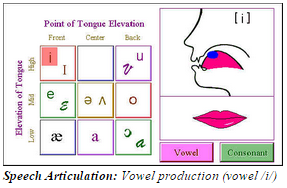
\includegraphics[totalheight=0.2\textheight]{speech-therapy.PNG}
    \caption{Speech Therapy 5 [Online image].}
    \cite{speechtherapy5:img}
    \label{fig:speechtherapy}
\end{figure}

\subsection{Video Voice}
Video Voice is a speech training software developed by Micro Video Corporation. It is a speech development tool which offers a wide variety of entertaining and motivating games in order for the student to learn. It provides visual feedback on pitch, volume, and vowel production. In \figref{fig:video-voice-1}, a plane supplying resources to small houses will move from the left to the right of the screen. The trainee must produce any sound as the plane flies directly above a house in order for the plane to drop the load. In \figref{fig:video-voice-2}, the red enemy spaceship flies up and down the screen, the trainee must control the volume of their speech in order to move the trainee's spaceship up and down, the louder the volume, the higher the spaceship flies. The trainee must place the spaceship in a way that it faces the enemy spaceship in order to destroy it.

\begin{figure}[h]
    \centering
    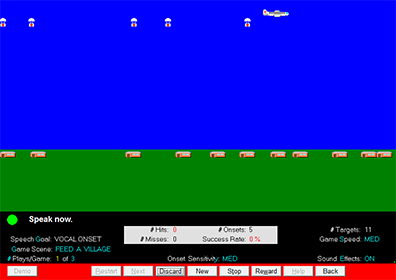
\includegraphics[totalheight=0.2\textheight]{video-voice-1.png}
    \caption{Video Voice}
    \label{fig:video-voice-1}
\end{figure}

\begin{figure}[h]
    \centering
    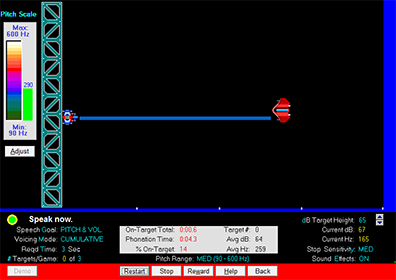
\includegraphics[totalheight=0.2\textheight]{video-voice-2.png}
    \caption{Video Voice}
    \label{fig:video-voice-2}
\end{figure}

\pagebreak

\subsection{Summary Table}
Table \ref{tab:comparisontable2} provides a summary of speech training software that were reviewed.
\begin{table}[h!]   %t means place on top, replace with b if you want to place at the bottom
\centering
\caption{Table of Comparison} \vspace{0.25em}
\begin{tabular}{|p{1.5in}|p{2in}|p{2in}|}
 \hline
\centering
Name of Software & Features & Means of Visual Feedback \\ \hline
	SpeechViewer
		& Provides a dozen exercises for the user; clear and immediate feedback; provides animated rewards during successful responses 
		& Visual and auditory feedback. Goal oriented feedback, if a goal is achieved, it indicates correct input.
		\\ \hline
	Speech Therapy 5
		& 70 voice-activated games; real-time feedback; aids in pitch, loudness, voiced and unvoiced phonation; voicing onset; maximum phonation time; sound and vowel tracking
		& Immediate animated feedback on the child's performance depending on the goal of the game.
		\\ \hline
	Video Voice
		& Wide variety of games; immediate feedback; aids in volume, pitch, and vowel production
		& Provides real-time feedback and immediately shows if the user is correct. A target is also employed which is hit by the user to indicate correct input. 
		\\ \hline
\end{tabular}
\label{tab:comparisontable2}
\end{table}